\chapter{Udviklingsproces}
Arbejdes forløbet har været præget af nogle forskellige arbejdes former, disse former vil blive beskrevet i detaljer hvordan gruppen har benyttet sig af dem.

\section{RUP}
\textbf{R}ational \textbf{U}nified \textbf{P}rocess er blevet anvendt til at holde den overordnet fremgangs metode til projektet.  

\begin{figure}[H]
	\centering
	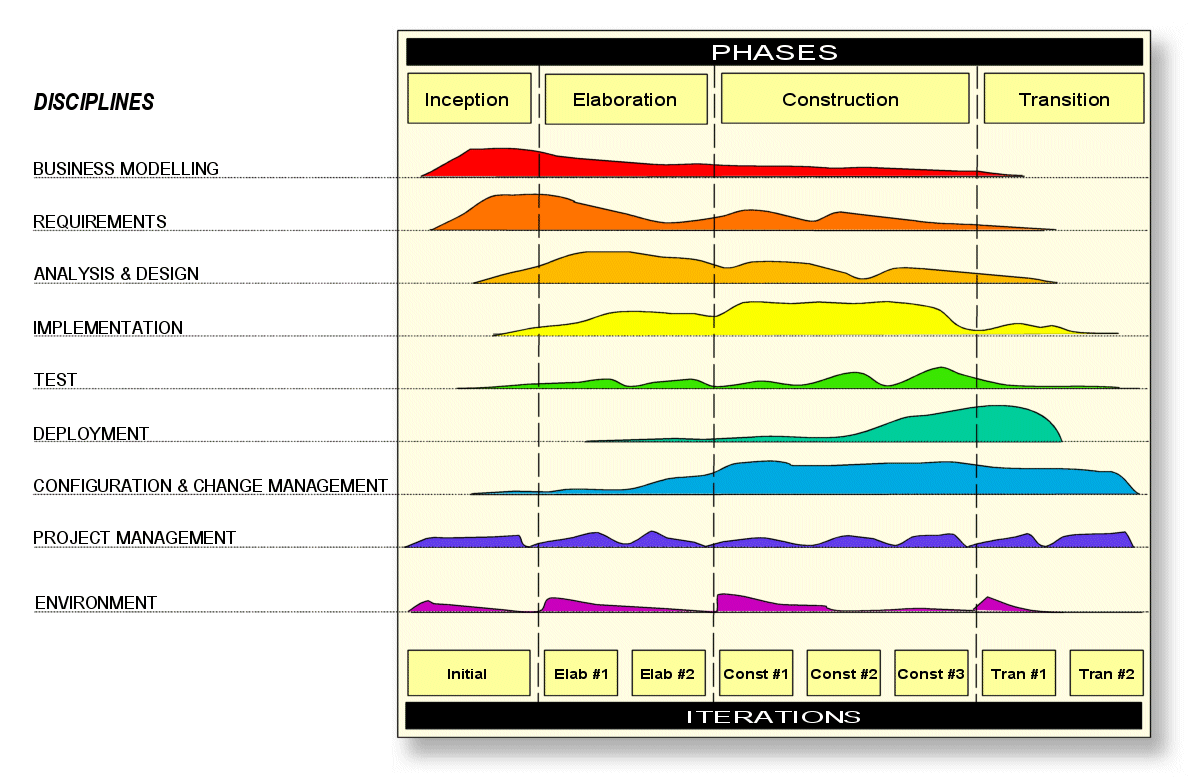
\includegraphics[width=0.60\textwidth]{Billeder/Udviklingsproces/RUP}
	\caption{RUP model}
	\label{fig:rup}
\end{figure}

\subsection{Inception}
I denne fase blev de indledende dokumenter udarbejdet. Der blev lavet forundersøgelse og valg vedrørende hardware. En indkøbs liste blev også udarbejdet i denne fase.  

\subsection{Elaboration}
I denne fase blev domain modellen udarbejdet, der blev fortaget en use case analyse af systemets funktionalitet. Krav til systemet blev også udarbejdet og det overordnet design til systemet blev udarbejdet. Ved brug af use case analysen blev der også udarbejdet en iterations plan over den kommende udvikling af systemet. 

\subsection{Construction}
I denne fase var produktet i fokus. Udviklingen forgik skiftevis mellem implementering af nyt funktionalitet, test og dokumentation af færdiggjort funktionalitet.

\subsection{Transition}
I denne fase blev der gjort opsamling af dokumentationen og rapporten samt accepttest.

\subsection{Dokument udarbejdelse}
Ved brug af RUP arbejdsmetoden blev der holdt et godt overblik over projektets fremgang og dokument håndtering. Som det kan ses på figur \ref{fig:dokument_udvikling} er dokumentationen opdelt i fire dokumenter, hvilket giver et godt overblik over de forskellige dokumenter tilhørende projektet.

\begin{figure}[H]
	\centering
	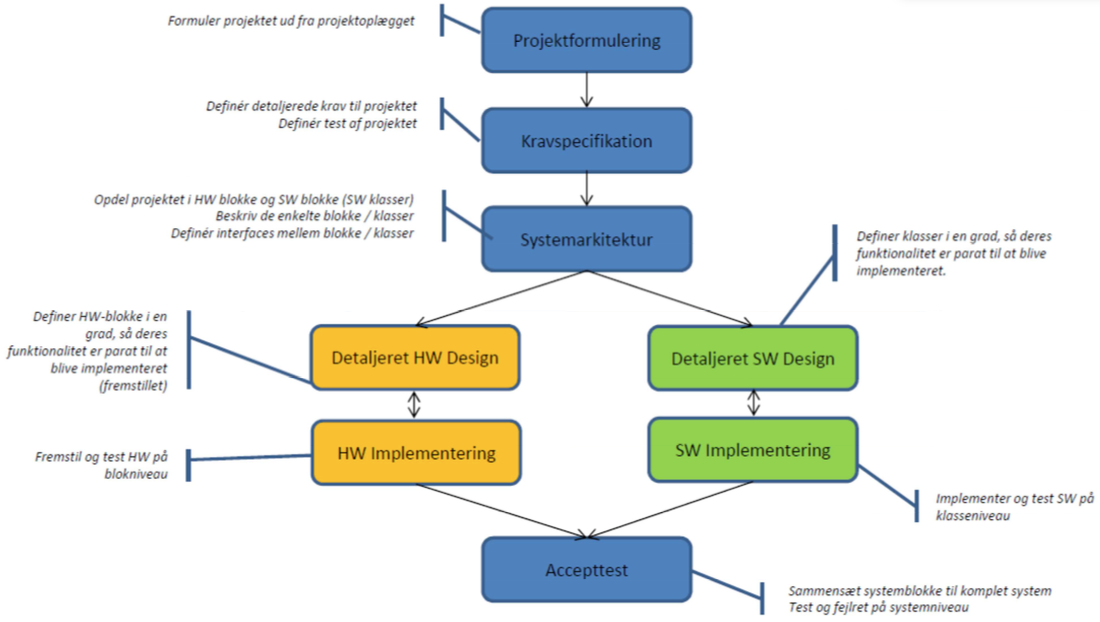
\includegraphics[width=0.75\textwidth]{Billeder/Udviklingsproces/Dokument_udvikling}
	\caption{Dokument udvikling}
	\label{fig:dokument_udvikling}
\end{figure}

\section{Iterativt udvikling}
Da projektet blev opdelt i use cases var det meget naturligt at opdele projektet i iterationer og derved starte med det mest grundlæggende funktionalitet først. Der blev planlagt fire iterationer. 

\textbf{Iteration 1}
